\subsection{Cache}\label{cache}
\emph{Drupal} maakt gebruik van \emph{caching} functionaliteit. Het doel van \emph{caching} is de website sneller maken. De cache slaat bijvoorbeeld pagina's op in de database. Op deze manier kan de website, gebruikmakend van de cache, de al eerder opgeslagen pagina een stuk sneller tonen. 

Na het wijzigen van bijvoorbeeld content of menu-items moet de cache handmatig verschoont worden, indien je de wijzigingen \emph{direct} zichtbaar wilt maken. 

\textbf{Cache opschonen:}

\begin{enumerate}
\item Ga naar  \drupalpath{admin/config/development/performance}.
\item Klik op de knop \emph{Alle caches legen}.
\item Wacht op de succes melding, dit duurt ongeveer een halve minuut.
\end{enumerate}

\begin{center}
	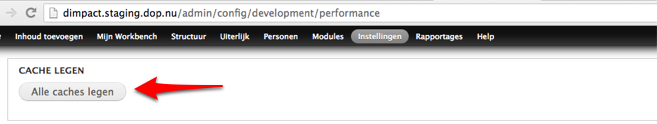
\includegraphics[width=\textwidth]{img/cache.png}
\end{center}